\documentclass[10pt]{article}         %% What type of document you're writing.
\usepackage{graphicx}
\usepackage{hyperref}
\usepackage[dvipsnames]{xcolor}

%%%%% Preamble

%% Packages to use

\usepackage{amsmath,amsfonts,amssymb}   %% AMS mathematics macros

%% Title Information.

\title{Twitter Data Model}
\author{Adolfo Centeno}
%% \date{2 July 2004}           %% By default, LaTeX uses the current date

%%%%% The Document

\begin{document}

\maketitle

\begin{abstract}
This document implements the Twitter Data Model.
\end{abstract}

\section{Data Model Description}



\textcolor{red}{Usuarios} de twitter (\textcolor{green}{ idusuario, usuario, email, passwd, telefono, nombre } ) \\
\textcolor{red}{Tweets}  (\textcolor{green}{ idtweet, tweet, urlimagen} ) \\

Los Usuarios \textcolor{yellow}{escribe} Tweets 


\section{E-R Model}

Twitter...

\begin{figure}[h]
     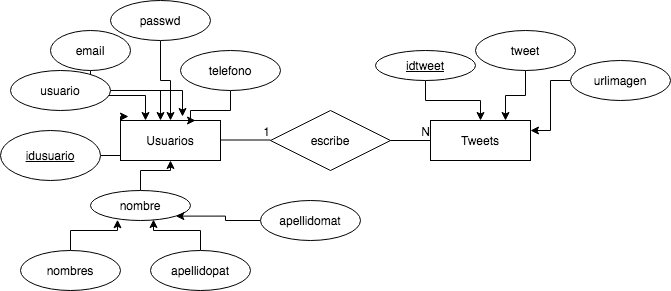
\includegraphics[scale=0.6]{er_twitter}
     \caption{Twitter E-R Model}
\end{figure}
   
\section{Relational Model}
Twitter Relational Model

\begin{figure}[h]
     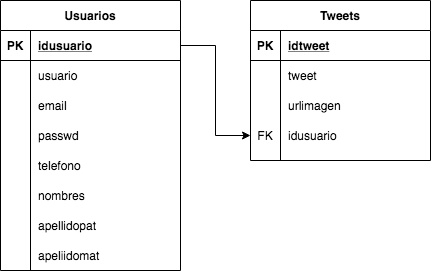
\includegraphics[scale=0.4]{relational_twitter}
     \caption{Twitter Relational Model}
\end{figure}


\section{Database in postgresql}
Database script

\begin{enumerate}

\item
	sudo -u postgres createdb adsoft\_twitter;
\item
	sudo -u postgres psql;
\item
	\textbackslash connect adsoft\_twitter;
\item
	create table usuarios(idusuario varchar(20), usuario varchar(20), email varchar(40), passwd varchar(8), telefono varchar(10), nombres varchar(20), apellidopat varchar(20), apellidomat varchar(20));
\item
	alter table usuarios add constraint pk\_idusuario primary key (idusuario);
\item
	insert into usuarios values('u1', 'adsoft', 'adsoft@live.com.mx', 'aa12', '2721908413', 'adolfo', 'centeno', 'tellez');
\item
	create table tweets(idtweet int, tweet varchar(130), urlimagen varchar(200), idusuario varchar(20));	
\item
	alter table tweets add constraint pk\_idtweet primary key(idtweet);
\item
	alter table tweets add constraint fk\_idtweet\_idusuario foreign key(idusuario) references usuarios(idusuario);
\item
	insert into tweets values (1, 'hola todos', 'myurl.jpg', 'u1'); \\
	insert into tweets values (2, 'hola todos', 'myurl.jpg', 'u2'); \\

\end{enumerate}
\end{document}

